\section*{Algebraic Closures}

\defn. \note{Algebraic Closure} Let \(E\) be an extension field of \(F\).
\begin{center}
    \(\bar{F}_E = \{\alpha \in E : \alpha \text{ is algebraic over } F\}\)
\end{center}
is called the \textbf{algebraic closure of \(F\) in \(E\)}.

\prop. \(\bar{F}_E\) is a field, and \(F \leq \bar{F}_E\).

\pf It is enough to show that \(\alpha \pm \beta\), \(\alpha \beta\), \(\alpha / \beta\) (\(\beta \neq 0\)) are in \(\bar{F}_E\) for all \(\alpha, \beta \in \bar{F}_E\). Associativity, commutativity and the distributive property directly follows since \(E\) is a field.

Consider \(F(\alpha, \beta) \subset E\). \(\alpha, \beta\) are algebraic over \(F\), so \(F(\alpha, \beta)\) is a finite extension and also an algebraic extension. Thus all elements of \(F(\alpha, \beta)\) are algebraic over \(F\), and \(F(\alpha, \beta) \subset \bar{F}_E\). The result directly follows. \qed

\defn. \note{Algebraically Closed Field}
\begin{enumerate}
    \item A field \(F\) is \textbf{algebraically closed} if every non-constant polynomial in \(F[x]\) has a zero in \(F\).
    \item \(\bar{F}\) is the \textbf{algebraic closure of \(F\)}, which is an algebraic extension field of \(F\) such that every non-constant polynomial in \(\bar{F}[x]\) has a zero in \(\bar{F}\).
\end{enumerate}

\(\bar{F}\) is a field containing all zeros of \(F[x]\). Does it actually exist? We need Zorn's lemma to construct the algebraic closure.

\defn. \note{Partially Ordered Set} \((S, \leq)\) is a \textbf{partially ordered set} if
\begin{enumerate}
    \item (Reflexive) \(\forall s \in S\), \(s \leq s\).
    \item (Anti-symmetric) \(\forall a, b \in S\), if \(a \leq b\) and \(b \leq a\), then \(a = b\).
    \item (Transitive) \(\forall a, b, c \in S\), if \(a \leq b\) and \(b \leq c\), then \(a \leq c\).
\end{enumerate}

\defn. \note{Chain} Let \(S\) be a partially ordered set. \(T \subset S\) is a \textbf{chain} if
\begin{center}
    \(\forall a, b \in T\), \(a \leq b\) or \(b \leq a\).
\end{center}
i.e, we can compare any two elements of \(T\).

\lemma. \note{Zorn} Let \(S\) be a partially ordered set. If every chain \(T \subset S\) has an upper bound in \(S\), then \(S\) has at least one maximal element.

\pf Equivalent to the Axiom of Choice. \qed

To use Zorn's lemma, we need to define a partially ordered set, and show that every chain has an upper bound. Finally, we should check if the maximal element of \(S\) can indeed be called the algebraic closure.

\thm. Every field has an algebraic closure \(\bar{F}\).

\pf Let \(S\) be the set of all algebraic extensions of \(F\).\footnote{\textit{Is \(S\) actually a set? Does it actually exist?}} We define a relation \(\leq\) as the following. For \(E_i, E_j \in S\), \(E_i \leq E_j \iff E_i \subset E_j\). It can be checked that \(S\) is a partially ordered set.

Let \(T = \{E_j : j \in J\}\) be a chain in \(S\), and take \(W = \bigcup_{E \in T} E\). \(W\) is an upper bound by definition, so we must show that \(W \in S\). We will show that (i) \(W\) is a field, and (ii) \(W\) is an algebraic extension field of \(F\).

\note{i} Suppose that \(\alpha \subset E_i\), \(\beta \subset E_j\) where \(E_i \subset E_j\) in \(T\). Then \(\alpha, \beta \in E_j\), where \(E_j\) is a field. So \(\alpha \pm \beta\), \(\alpha\beta\), \(\alpha / \beta \in E_j \subset W\). \(W\) is a field.

\note{ii} Let \(\alpha \in W\). Then \(\alpha \in E\) for some \(E \in T\). \(E\) is an algebraic extension of \(F\), so \(\alpha\) is algebraic over \(F\), and thus \(W\) is an algebraic extension of \(F\).

By Zorn's lemma, take a maximal element \(\bar{F}\) of \(S\). We show that \(\bar{F}\) is algebraically closed.

Suppose not. Then there exists a irreducible polynomial in \(\bar{F}[x]\) having degree greater than 1. Let \(\alpha\) be a zero of \(f(x)\). \(\bar{F}(\alpha)\) is an algebraic extension of \(F\), so \(\bar{F} < \bar{F}(\alpha) \in S\), contradicting that \(\bar{F}\) is maximal. \qed

\pagebreak

\topic{Geometric Constructions}

We have a ruler and a compass. Rulers are used to draw or extend straight lines, and compasses are used to draw circles or copy lengths. We are also given a line segment, as a unit length.

\defn. \note{Constructible Real Number} A real number \(\alpha\) is \textbf{constructible} if we can construct a line segment of length \(\abs{\alpha}\) in a finite number of steps from a given segment of unit length by using a ruler and a compass.

It is easy to see that with the given unit length as \(1\), any integer is constructible. The following theorem shows that constructible real numbers form a field.

\thm. Let \(\alpha, \beta\) be constructible real numbers. Then
\[
    \alpha \pm \beta, \quad \alpha\beta, \quad \alpha / \beta\;\; (\beta \neq 0)
\]
are constructible.

\pf We are given lengths \(\alpha\), \(\beta\) and \(1\). \(\alpha \pm \beta\) is very simple.

As for constructing \(\alpha \beta\), refer to the diagram on the left. Start with given lengths \(OA = \alpha\) and \(OB = \beta\), with an arbitrary angle. Pick a point \(P\) with \(OP = 1\) on the line \(OB\). Then construct a line from \(B\) that is parallel to \(AP\). Let \(Q\) be the intersection of \(OA\) with this line. Then the triangles \(OAP\) and \(OQB\) are similar, thus
\[
    OA : OP = OQ : OB \implies OQ = OA \cdot OB = \alpha \beta.
\]

For \(\alpha / \beta\), refer to the diagram on the right. Similarly, start with given lengths \(OA = \alpha\) and \(OB = \beta\), with an arbitrary angle. Pick a point \(P\) with \(OP = 1\) on the line \(OB\). Then construct a line from \(P\) that is parallel to \(AB\). Let \(Q\) be the intersection of \(OA\) with this line. Then the triangles \(OPQ\) and \(OBA\) are similar, thus
\[
    OP : OQ = OB : OA \implies OQ = \frac{OA}{OB} = \frac{\alpha}{\beta}.
\]
\begin{center}

    \usetikzlibrary {decorations.pathmorphing, decorations.pathreplacing, decorations.shapes}
    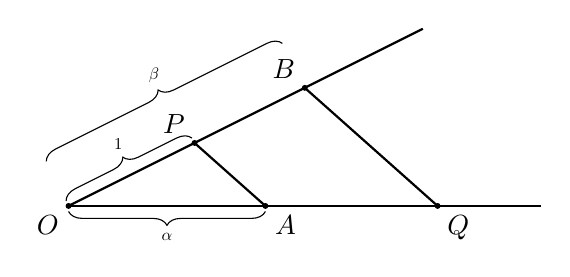
\begin{tikzpicture}
        \coordinate (O) at (0, 0);
        \node[below left] at (O) {\(O\)};

        \coordinate (A) at (2.5, 0);
        \node[below right] at (A) {\(A\)};

        \coordinate (B) at (3, 1.5);
        \node[above left] at (B) {\(B\)};

        \coordinate (P) at (1.6, 0.8);
        \node[above left] at (P) {\(P\)};

        \coordinate (Q) at (4.687, 0);
        \node[below right] at (Q) {\(Q\)};

        \filldraw[color=black] (O) circle (0.03);
        \filldraw[color=black] (A) circle (0.03);
        \filldraw[color=black] (B) circle (0.03);
        \filldraw[color=black] (P) circle (0.03);
        \filldraw[color=black] (Q) circle (0.03);

        \draw[thick] (O) -- (6, 0);
        \draw[thick] (O) -- (4.5, 2.25);
        \draw[thick] (P) -- (A);
        \draw[thick] (B) -- (Q);

        \draw[decorate,decoration={brace,raise=2pt,amplitude=5pt}] (O) -- (P)
            node[scale=0.6, midway, above=18pt, left=2pt] {\(1\)};
        \draw[decorate,decoration={brace,raise=18pt,amplitude=5pt}] (O) -- (B)
            node[scale=0.6, midway, above=43pt, left=13pt] {\(\beta\)};
        \draw[decorate,decoration={brace,mirror,raise=2pt,amplitude=5pt}] (O) -- (A)
            node[scale=0.6, midway, below=13pt] {\(\alpha\)};
    \end{tikzpicture}
    \qquad
    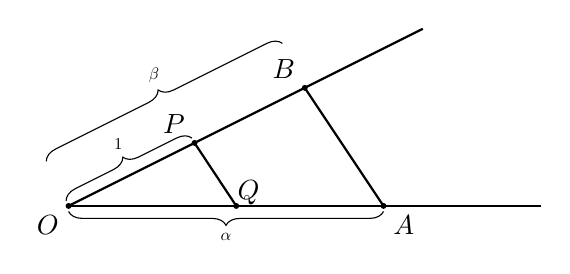
\begin{tikzpicture}
        \coordinate (O) at (0, 0);
        \node[below left] at (O) {\(O\)};

        \coordinate (A) at (4, 0);
        \node[below right] at (A) {\(A\)};

        \coordinate (B) at (3, 1.5);
        \node[above left] at (B) {\(B\)};

        \coordinate (P) at (1.6, 0.8);
        \node[above left] at (P) {\(P\)};

        \coordinate (Q) at (2.13, 0);
        \node[above right=-3pt] at (Q) {\(Q\)};

        \filldraw[color=black] (O) circle (0.03);
        \filldraw[color=black] (A) circle (0.03);
        \filldraw[color=black] (B) circle (0.03);
        \filldraw[color=black] (P) circle (0.03);
        \filldraw[color=black] (Q) circle (0.03);

        \draw[thick] (O) -- (6, 0);
        \draw[thick] (O) -- (4.5, 2.25);
        \draw[thick] (P) -- (Q);
        \draw[thick] (B) -- (A);

        \draw[decorate,decoration={brace,raise=2pt,amplitude=5pt}] (O) -- (P)
            node[scale=0.6, midway, above=18pt, left=2pt] {\(1\)};
        \draw[decorate,decoration={brace,raise=18pt,amplitude=5pt}] (O) -- (B)
            node[scale=0.6, midway, above=43pt, left=13pt] {\(\beta\)};
        \draw[decorate,decoration={brace,mirror,raise=2pt,amplitude=5pt}] (O) -- (A)
            node[scale=0.6, midway, below=13pt] {\(\alpha\)};
    \end{tikzpicture}
\end{center}

\rmk Since \(\Q\) is the smallest field containing \(\Z\), constructible real numbers contain \(\Q\). So constructible real numbers is an extension field of \(\Q\).

\pagebreak
